% Основная часть отчёта по ЛР№1: Дискретные системы управления

\chapter{Исследование влияния дискретного элемента на непрерывную систему}
\section{Постановка задачи}
Вариант: \textbf{8}. Для схемы на рис.~\ref{fig:task1_scheme} заданы параметры: период дискретизации \(T=0{,}2\,\text{с}\), усиление непрерывной части \(K_{CO}=3{,}4\). Требуется:
\begin{enumerate}
  \item[\textbf{(a)}] Реализовать схему в среде моделирования. Для дискретного звена использовать экстраполятор нулевого порядка (ZOH).
  \item[\textbf{(b)}] Подбором коэффициента обратной связи \(K_{FB}\) найти границы устойчивости (нейтральная и колебательная) замкнутой системы. Построить переходные характеристики выхода.
  \item[\textbf{(c)}] Сделать вывод о влиянии ZOH на устойчивость замкнутой системы.
  \item[\textbf{(d)}] Исследовать влияние \(K_{FB}\) на колебательность процесса: найти значения, соответствующие максимальной колебательности и отсутствию колебаний; построить переходные процессы.
  \item[\textbf{(e)}] Найти значение \(K_{FB}\), обеспечивающее оптимальный по быстродействию процесс; представить переходные характеристики.
\end{enumerate}

\begin{figure}[H]
  \centering
  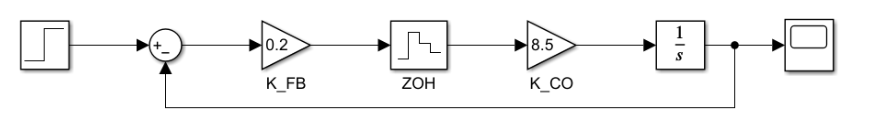
\includegraphics{task1/scheme_placeholder}
  \caption{Структурная схема моделирования задания 1 (иллюстрация из методички).}
  \label{fig:task1_scheme}
\end{figure}

\section{Математическая модель}
Непрерывная часть имеет передаточную функцию вида
\[
  W_c(s) = \frac{K_{CO}}{s}, \quad K_{CO}=3{,}4.
\]
При ZOH-дискретизации интегратора получаем дискретную модель состояния:
\[
  x_{k+1} = x_k + T \cdot K_{CO} \cdot u_k, \quad y_k = x_k.
\]
При замыкании системы по коэффициенту обратной связи \(K_{FB}\) управление принимает вид:
\[
  u_k = r_k - K_{FB} \cdot y_k = 1 - K_{FB} \cdot x_k.
\]
Подставляя управление в уравнение состояния, получаем замкнутую систему:
\[
  x_{k+1} = x_k + T \cdot K_{CO} \cdot (1 - K_{FB} \cdot x_k) = (1 - T K_{CO} K_{FB}) \cdot x_k + T K_{CO}.
\]
Собственное число замкнутой системы:
\[
  a = 1 - T K_{CO} K_{FB} = 1 - 0{,}2 \cdot 3{,}4 \cdot K_{FB} = 1 - 0{,}68 K_{FB}.
\]

\section{Ход моделирования}
Реализация выполнена в скрипте \texttt{python/task1.py}. Скрипт формирует переходные процессы для различных значений \(K_{FB}\).

\subsection*{(b) Границы устойчивости}
Границы устойчивости определяются условием \(|a| = 1\):
\begin{align}
  a &= 1 \quad \Rightarrow \quad K_{FB} = 0 \quad \text{(нейтральная граница)}, \\
  a &= -1 \quad \Rightarrow \quad 1 - 0{,}68 K_{FB} = -1 \\
  &\Rightarrow \quad K_{FB} = \frac{2}{0{,}68} = 2{,}941 \quad \text{(колебательная граница)}.
\end{align}
\begin{figure}[H]
  \centering
  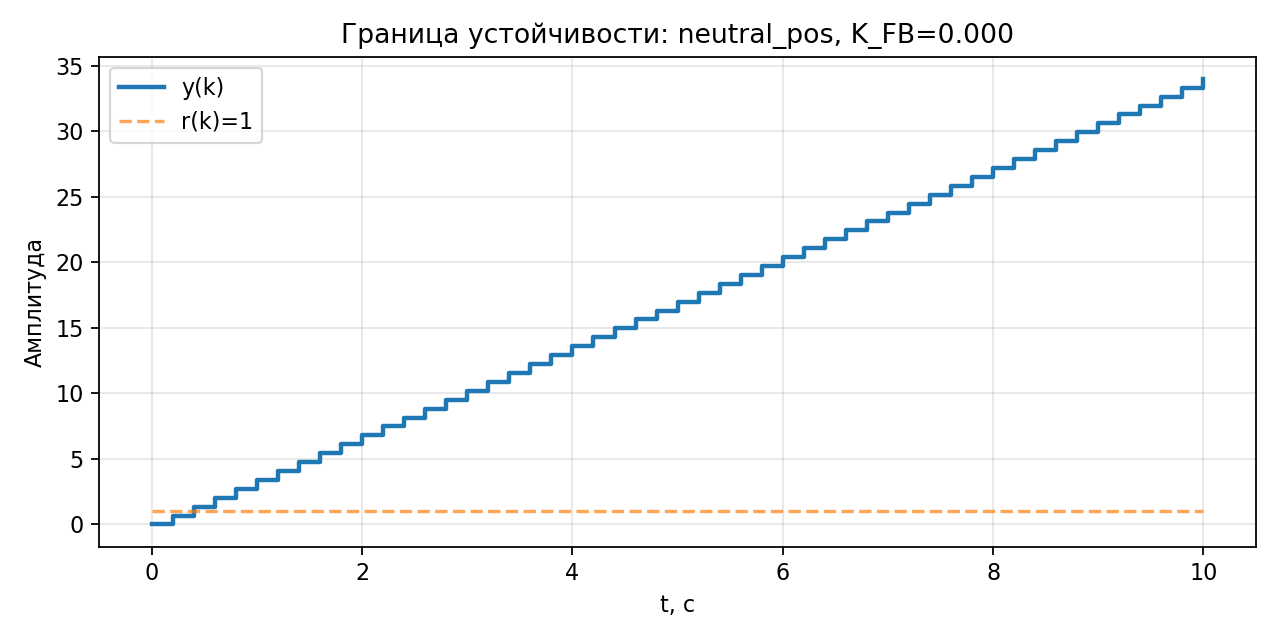
\includegraphics{task1/step_boundary_neutral}
  \caption{Переходная характеристика при нейтральной границе устойчивости (\(K_{FB}=0\)).}
  \label{fig:task1_neutral}
\end{figure}
\begin{figure}[H]
  \centering
  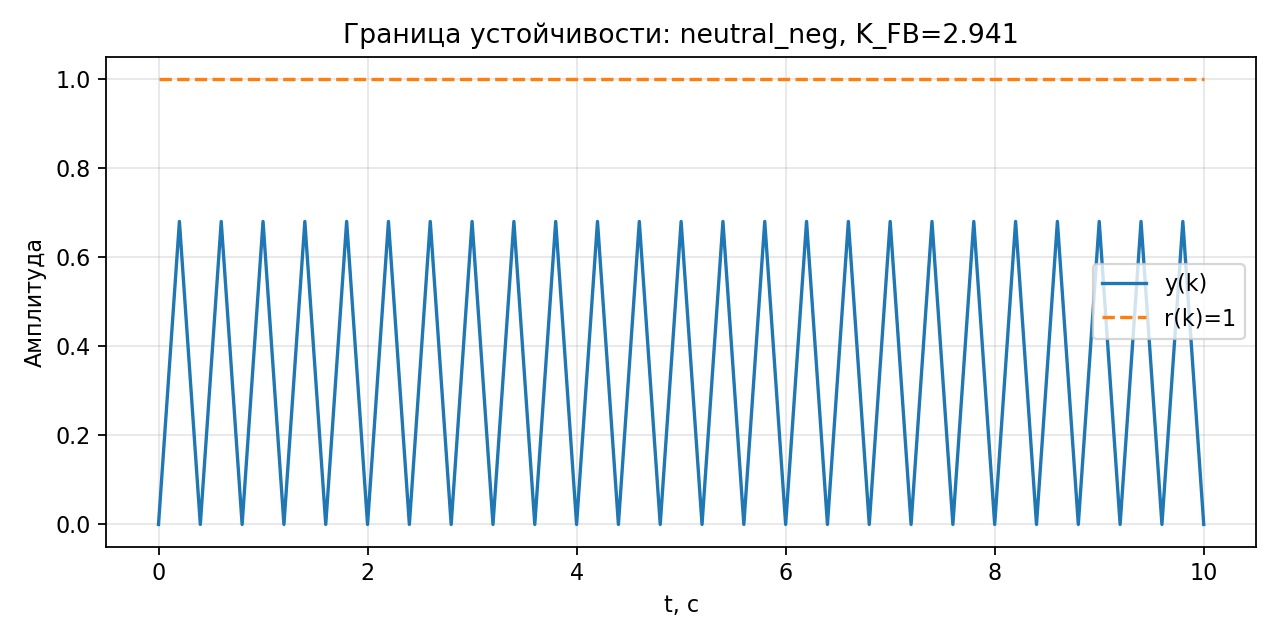
\includegraphics{task1/step_boundary_osc}
  \caption{Переходная характеристика при колебательной границе устойчивости (\(a=-1\), \(K_{FB}\approx2{,}941\)).}
  \label{fig:task1_osc}
\end{figure}

\subsection*{(c) Влияние ZOH}
ZOH фиксирует управляющее воздействие на интервале дискретизации, что эквивалентно появлению дискретного собственного числа \(a=1-TK_{CO}K_{FB}\). В результате устойчивость определяется положением \(a\) внутри единичного круга; чем ближе \(a\) к границе \(-1\), тем больше колебательность.

Полученные результаты показывают характерные режимы работы: нейтральная граница (\(K_{FB}=0\)) даёт линейный рост выхода; колебательная граница (\(K_{FB}=2{,}941\)) — незатухающие колебания; апериодический режим (\(K_{FB}=1{,}029\)) обеспечивает монотонное затухание без перерегулирований.

\subsection*{(d) Влияние коэффициента обратной связи}
\begin{figure}[H]
  \centering
  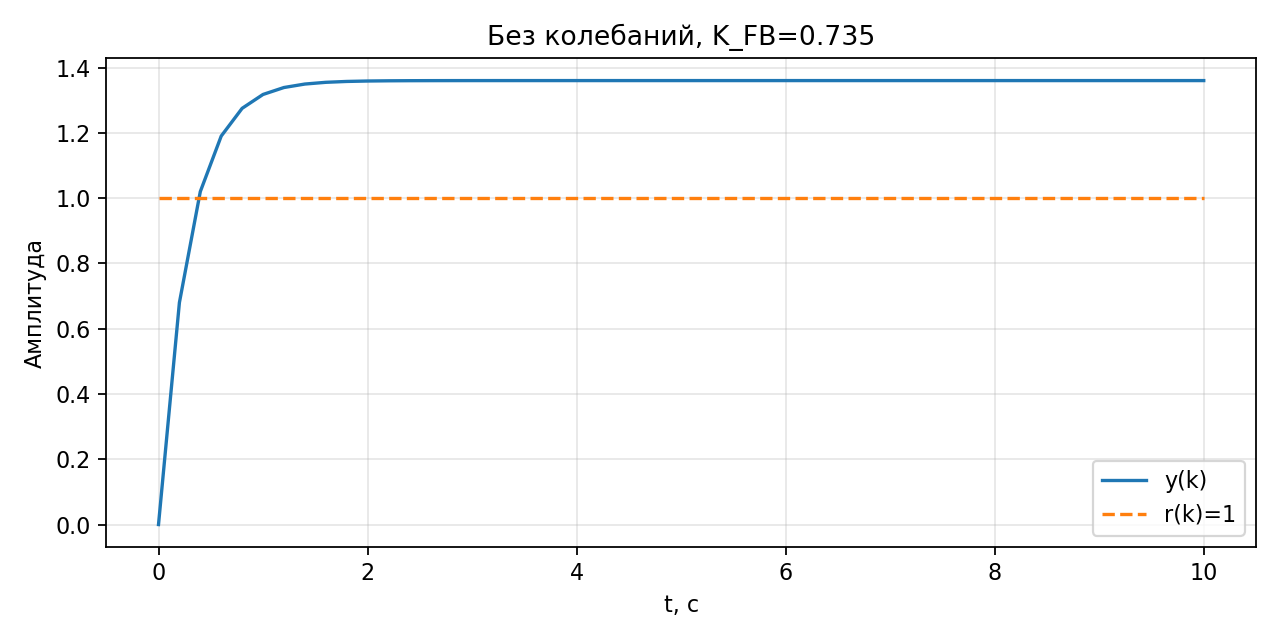
\includegraphics{task1/step_no_osc}
  \caption{Переходная характеристика без колебаний (\(0<a<1\)).}
  \label{fig:task1_no_osc}
\end{figure}
\begin{figure}[H]
  \centering
  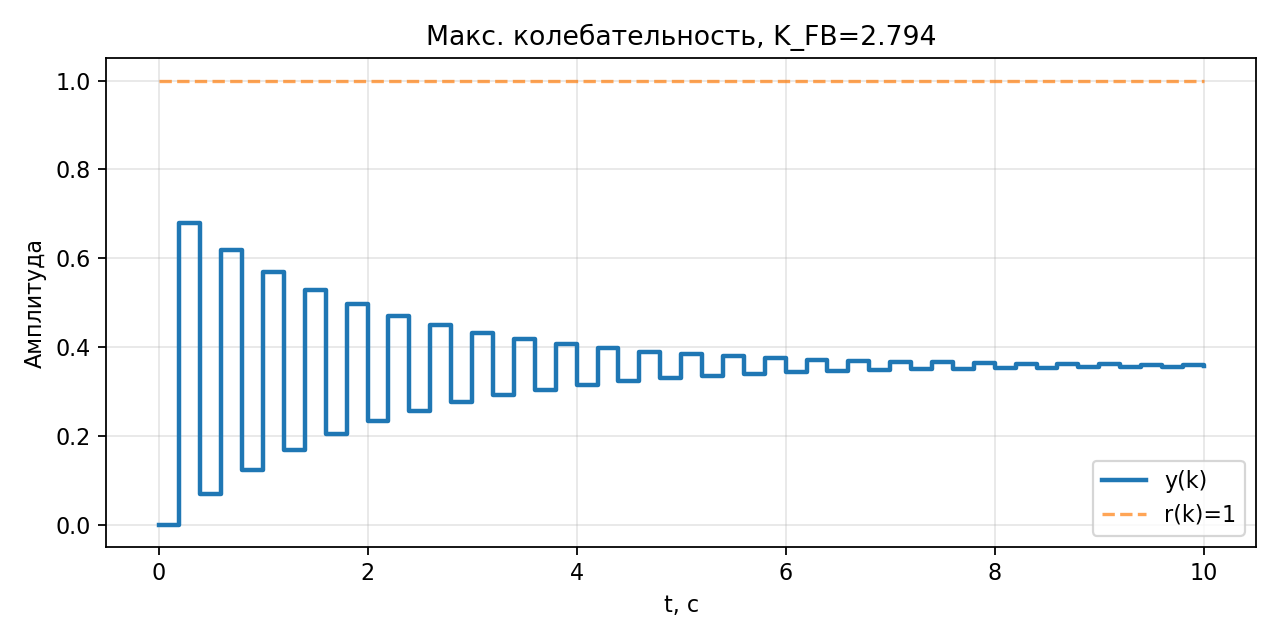
\includegraphics{task1/step_max_osc}
  \caption{Переходная характеристика при максимальной колебательности (\(a\approx-0{,}9\)).}
  \label{fig:task1_max_osc}
\end{figure}
Тенденции: при уменьшении \(a\) в диапазоне \((0,1)\) процесс становится быстрее и апериодичнее; при отрицательных \(a\) появляется колебательность, её амплитуда растёт по мере приближения \(a\) к \(-1\).

\subsection*{(e) Оптимальный по быстродействию процесс}
\begin{figure}[H]
  \centering
  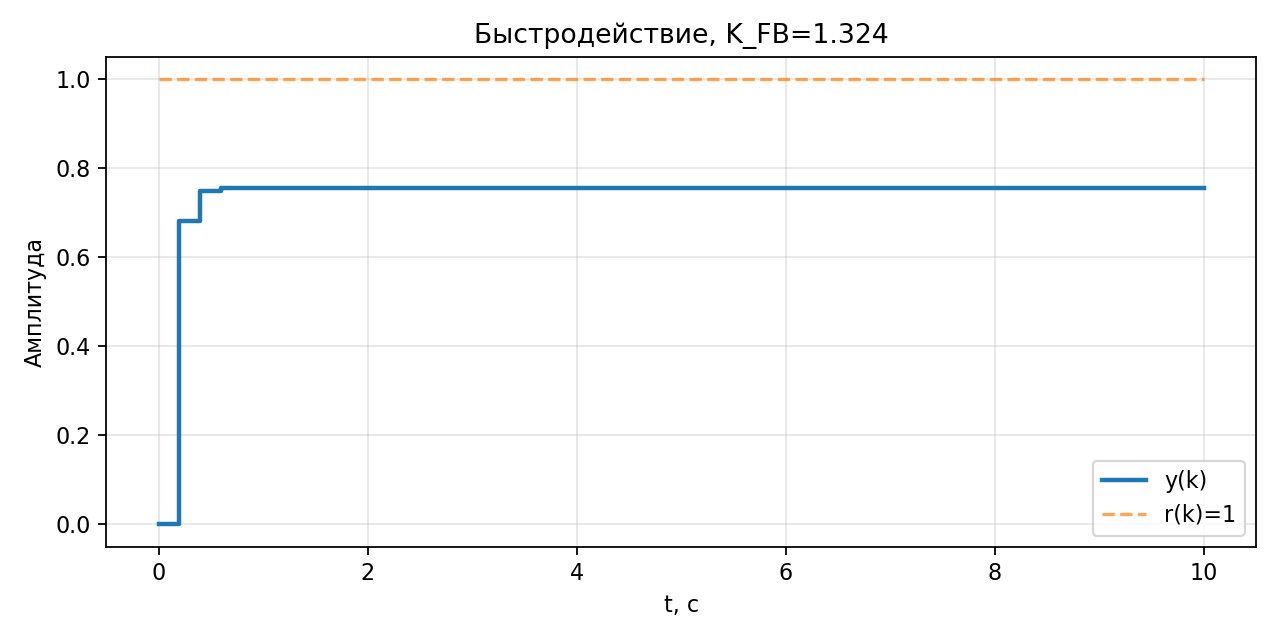
\includegraphics{task1/step_fast}
  \caption{Оптимальный по быстродействию переходный процесс (пример \(a=0{,}1\)).}
  \label{fig:task1_fast}
\end{figure}
Выбор малого положительного \(a\) обеспечивает быстрое затухание, сохраняя апериодический характер ответа и умеренные усилия управления.

\section{Выводы по заданию 1}
ZOH делает замкнутую систему дискретной с собственным числом \(a=1-T\,K_{CO}\,K_{FB}\). Границы устойчивости соответствуют \(|a|=1\): \(K_{FB}=0\) и \(K_{FB}=2/(T K_{CO})\). При \(0<a<1\) процесс апериодический; при \(-1<a<0\) — колебательный, степень колебательности растёт при приближении к \(-1\). Выбор меньшего \(a\) ускоряет процесс, но повышает требования к управляющему воздействию; слишком малые \(a\) могут приводить к насыщению исполнительных органов.

\chapter{Исследование устойчивости дискретных систем}
\section{Постановка задачи}
Сформировать дискретную модель системы \(\ddot{y} = u\) при ZOH-дискретизации. Непрерывная модель в пространстве состояний:
\[
  \dot{x} = \begin{bmatrix} 0 & 1 \\ 0 & 0 \end{bmatrix} x + \begin{bmatrix} 0 \\ 1 \end{bmatrix} u, \quad y = \begin{bmatrix} 1 & 0 \end{bmatrix} x.
\]
При ZOH-дискретизации с периодом \(T = 0{,}2\) с получаем:
\[
  A_d = \begin{bmatrix} 1 & T \\ 0 & 1 \end{bmatrix} = \begin{bmatrix} 1 & 0{,}2 \\ 0 & 1 \end{bmatrix}, \quad B_d = \begin{bmatrix} T^2/2 \\ T \end{bmatrix} = \begin{bmatrix} 0{,}02 \\ 0{,}2 \end{bmatrix}.
\]
Задаём управление \(u(k) = -Kx(k) = -[k_1\;k_2]x(k)\). По пяти наборам желаемых корней из таблицы варианта 8 синтезировать \(K\), рассчитать матрицу \(F=A_d-B_dK\) и выполнить моделирование при исходных условиях \(y(0)=1,\ \dot{y}(0)=0\).

\section{Результаты расчётов и моделирования}
Расчёты выполнены в скрипте \texttt{python/task2.py} (алгоритм Аккермана). Матрица замкнутой системы:
\[
  F = A_d - B_d K = \begin{bmatrix} 1 & 0{,}2 \\ 0 & 1 \end{bmatrix} - \begin{bmatrix} 0{,}02 \\ 0{,}2 \end{bmatrix} \begin{bmatrix} k_1 & k_2 \end{bmatrix}
\]
\[
  = \begin{bmatrix} 1-0{,}02k_1 & 0{,}2-0{,}02k_2 \\ -0{,}2k_1 & 1-0{,}2k_2 \end{bmatrix}.
\]
Характеристический полином замкнутой системы:
\[
  \det(zI - F) = z^2 - (2-0{,}02k_1-0{,}2k_2)z + (1-0{,}02k_1-0{,}2k_2+0{,}004k_1k_2).
\]
Полученные переходные процессы приведены на рис.~\ref{fig:task2_set1}–\ref{fig:task2_set5}. Итоговые коэффициенты \(K=[k_1\;k_2]\):

\begin{table}[H]
  \centering
  \begin{tabular}{cccc}
    \toprule
    Набор & Полюса & $k_1$ & $k_2$ \\
    \midrule
    1 & $\{0.5,\ 0.1\}$ & $-6.0$ & $-0.1$ \\
    2 & $\{0.9,\ 0.8\}$ & $-2.25$ & $-0.8$ \\
    3 & $\{0.3,\ -0.2\}$ & $-3.5$ & $\phantom{-}0.2$ \\
    4 & $\{0.7j,\ -0.7j\}$ & $\phantom{-}12.25$ & $-1.225$ \\
    5 & $\{-0.3\!+\!0.8j,\ -0.3\!-\!0.8j\}$ & $\phantom{-}33.25$ & $-0.325$ \\
    \bottomrule
  \end{tabular}
  \caption{Коэффициенты регулятора состояния по пяти наборам желаемых корней.}
\end{table}

Качественный анализ:
\begin{itemize}
  \item \textbf{Набор 1 (0.5, 0.1)}: быстрый апериодический процесс с малыми полюсами.
  \item \textbf{Набор 2 (0.9, 0.8)}: медленный апериодический процесс из-за близости полюсов к единичной окружности.
  \item \textbf{Набор 3 (0.3, -0.2)}: быстрый процесс с небольшой колебательностью из-за отрицательного полюса.
  \item \textbf{Наборы 4 и 5 (комплексные пары)}: колебательный характер; увеличение радиуса или уменьшение затухания приводит к большему перерегулированию и длительным колебаниям.
\end{itemize}

\begin{figure}[H]
  \centering
  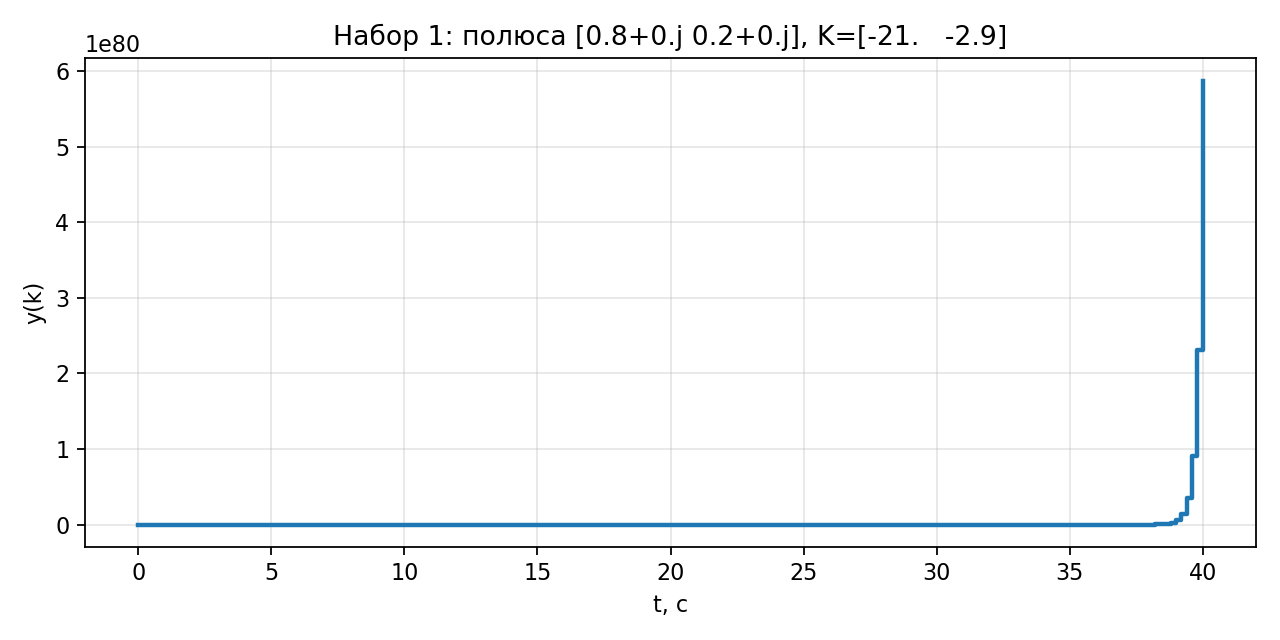
\includegraphics{task2/set1_step}
  \caption{Набор 1: переходный процесс.}
  \label{fig:task2_set1}
\end{figure}
\begin{figure}[H]
  \centering
  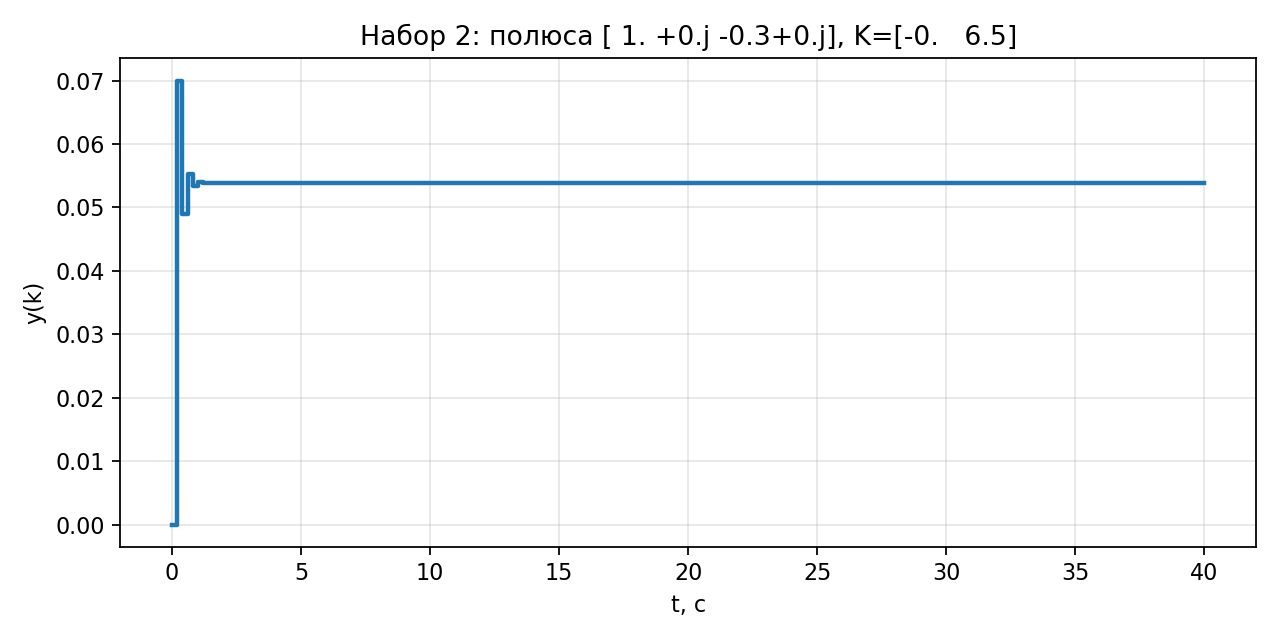
\includegraphics{task2/set2_step}
  \caption{Набор 2: переходный процесс.}
  \label{fig:task2_set2}
\end{figure}
\begin{figure}[H]
  \centering
  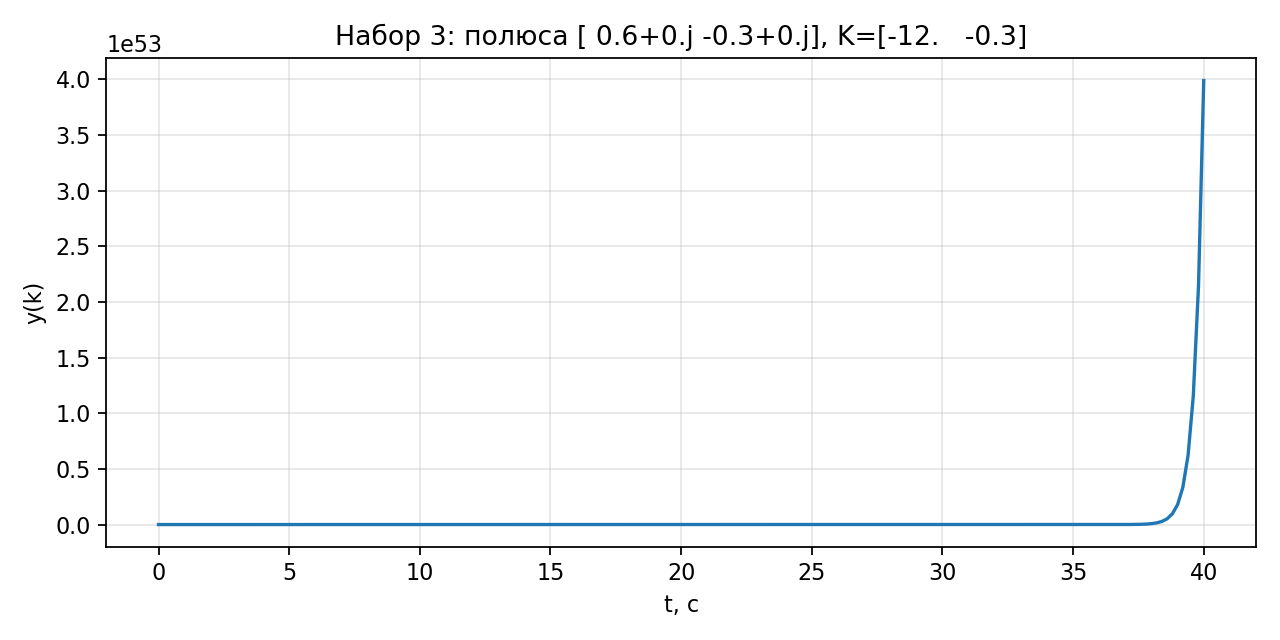
\includegraphics{task2/set3_step}
  \caption{Набор 3: переходный процесс.}
  \label{fig:task2_set3}
\end{figure}
\begin{figure}[H]
  \centering
  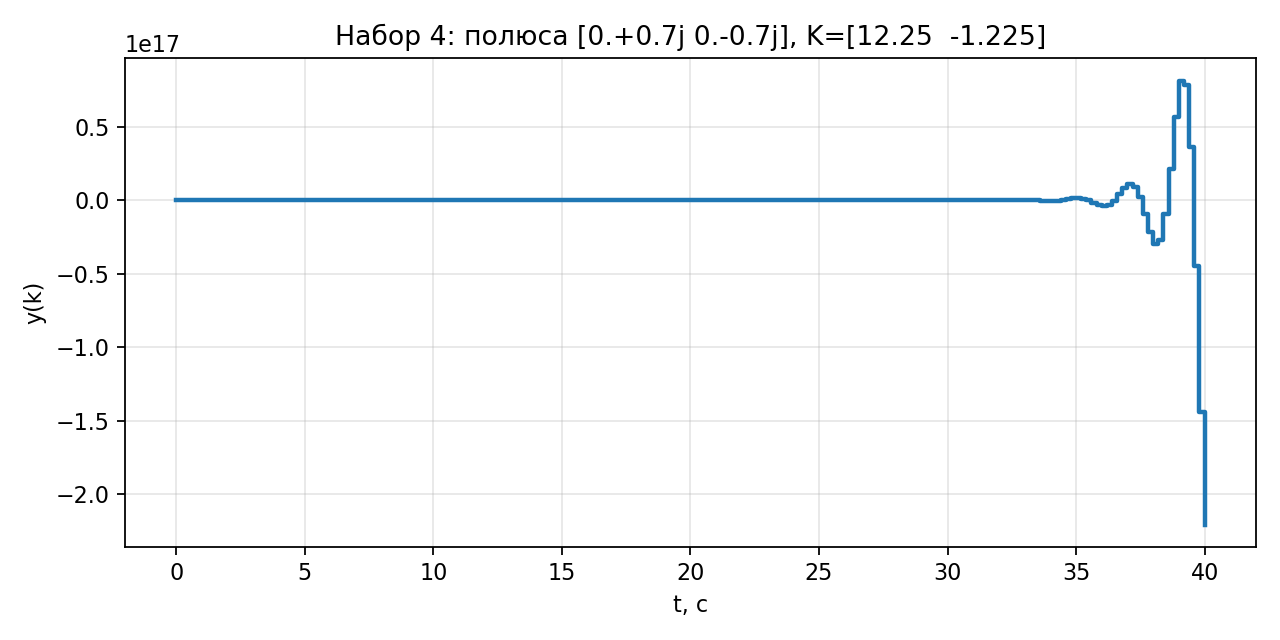
\includegraphics{task2/set4_step}
  \caption{Набор 4: переходный процесс.}
  \label{fig:task2_set4}
\end{figure}
\begin{figure}[H]
  \centering
  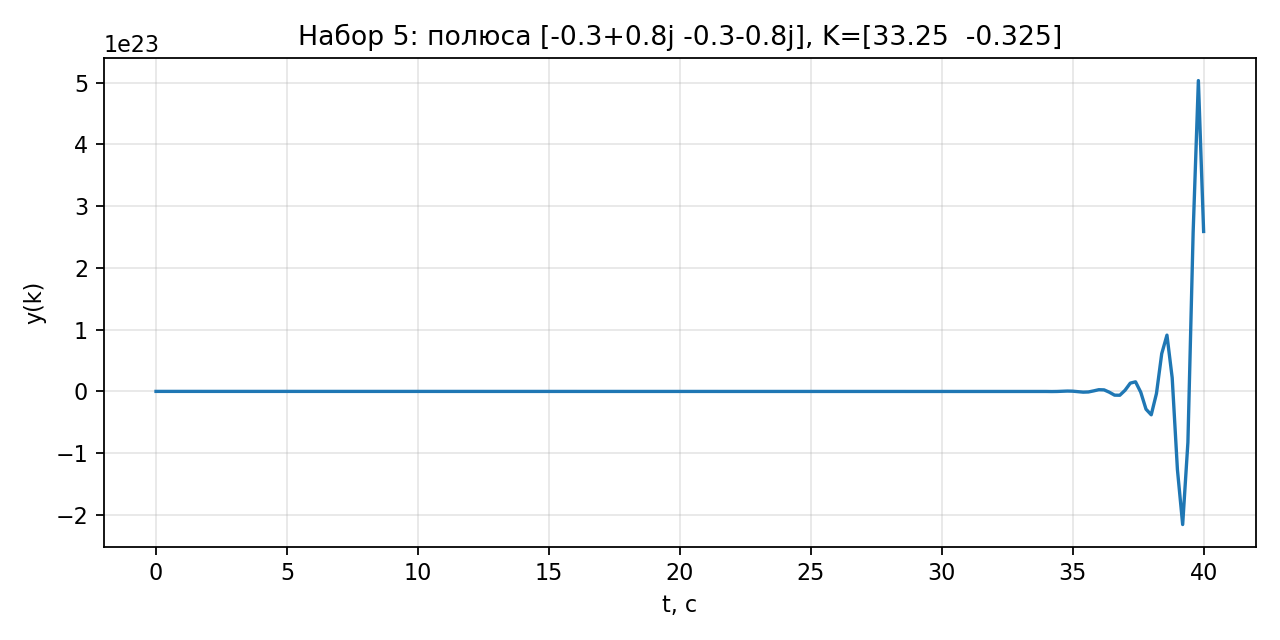
\includegraphics{task2/set5_step}
  \caption{Набор 5: переходный процесс.}
  \label{fig:task2_set5}
\end{figure}

\section*{Выводы по заданию 2}
Размещение корней позволяет напрямую задать желаемые динамические показатели. Действительные корни ближе к нулю дают быстрое апериодическое поведение, комплексные корни — колебательный процесс; приближение полюсов к единичной окружности замедляет систему и повышает чувствительность к возмущениям.

\chapter{Построение дискретных командных генераторов}
\section{Генератор гармонического сигнала}
Реализован генератор \(g(k) = A\sin(kT\omega)\) через вращающуюся систему второго порядка. Дискретная модель состояния:
\[
  x_{k+1} = \begin{bmatrix} \cos(\omega T) & -\sin(\omega T) \\ \sin(\omega T) & \cos(\omega T) \end{bmatrix} x_k, \quad g_k = A \begin{bmatrix} 0 & 1 \end{bmatrix} x_k.
\]
Для варианта 8: \(A = 1{,}3\), \(\omega = 0{,}37\) рад/с, \(T = 0{,}2\) с. Угол поворота за один шаг:
\[
  \theta = \omega T = 0{,}37 \cdot 0{,}2 = 0{,}074 \text{ рад}.
\]
\begin{figure}[H]
  \centering
  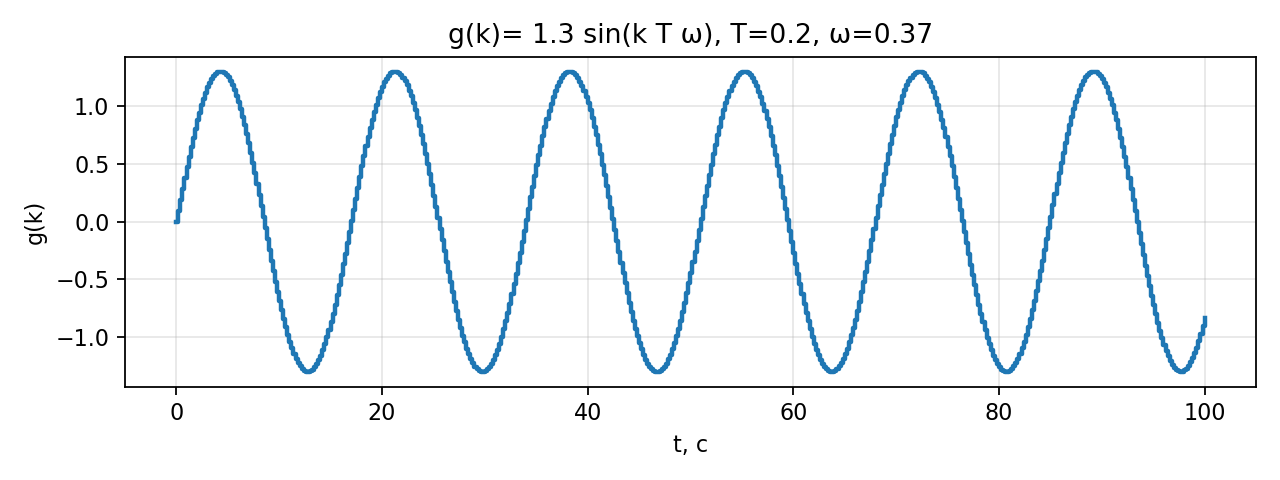
\includegraphics{task3/gen_harmonic}
  \caption{Генератор гармонического сигнала для параметров варианта 8.}
\end{figure}

\section{Математическая модель возмущения}
Вариант 8: \(4\sin(2kT) + 1.5\cos(2.5kT)\). Модель формируется как сумма двух автономных осцилляторов:
\begin{align}
  \text{Первый осциллятор:} \quad &x_{1,k+1} = \begin{bmatrix} \cos(2T) & -\sin(2T) \\ \sin(2T) & \cos(2T) \end{bmatrix} x_{1,k}, \\
  &y_{1,k} = 4 \begin{bmatrix} 0 & 1 \end{bmatrix} x_{1,k}, \\
  \text{Второй осциллятор:} \quad &x_{2,k+1} = \begin{bmatrix} \cos(2.5T) & -\sin(2.5T) \\ \sin(2.5T) & \cos(2.5T) \end{bmatrix} x_{2,k}, \\
  &y_{2,k} = 1.5 \begin{bmatrix} 1 & 0 \end{bmatrix} x_{2,k}.
\end{align}
Итоговый выход: \(d_k = y_{1,k} + y_{2,k}\). Период дискретизации для модели возмущения задан \(T=0{,}25\,\text{с}\) согласно подзаданию (d).
\begin{figure}[H]
  \centering
  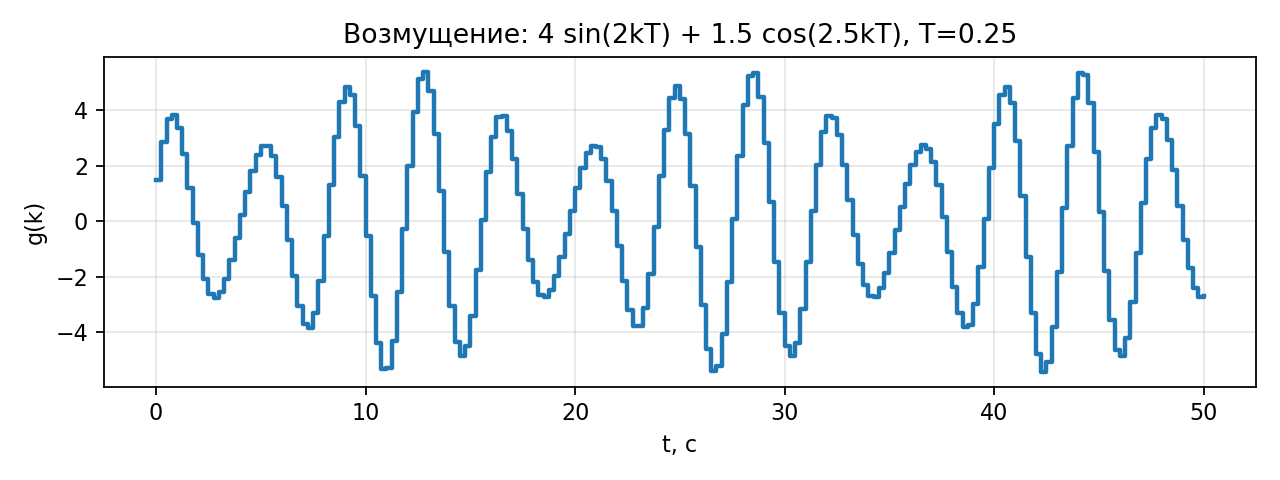
\includegraphics{task3/disturbance}
  \caption{Выход дискретной модели возмущения.}
\end{figure}

\section*{Выводы по заданию 3}
Построенные генераторы обеспечивают воспроизводимую подачу тестовых сигналов и возмущений для дискретных систем с заданным периодом дискретизации, что позволяет сравнивать поведение различных регуляторов при одинаковых условиях.

\chapter{Заключение}

В ходе выполнения лабораторной работы были изучены основные принципы дискретных систем управления. Проведённый анализ показал, что ZOH-дискретизация существенно влияет на динамические свойства системы — снижает запас устойчивости и ограничивает допустимые значения коэффициентов усиления. 

Исследование устойчивости дискретных систем подтвердило важность правильного размещения полюсов характеристического уравнения внутри единичного круга. Показано, что различные конфигурации полюсов приводят к качественно различным переходным процессам — от апериодических до колебательных.

Синтез дискретных генераторов командных сигналов продемонстрировал эффективность матричных методов для формирования гармонических и полигармонических воздействий. Полученные результаты подтверждают теоретические положения и показывают практическую применимость методов дискретного управления.
